\chapter{Introdução}
A mortalidade infantil é um problema social que ocorre em escala global e a redução
dela faz parte das Metas do Desenvolvimento do Milênio, compromisso assumido pelos países
integrantes da Organização das Nações Unidas (ONU), do qual o Brasil é signatário.

A taxa de mortalidade infantil consiste na relação entre o óbito de crianças no primeiro ano
de vida e a quantidade de nascidos vivos do mesmo período. Para facilidade de comparação entre
os diferentes países ou regiões do globo esta taxa é normalmente expressa em número de óbitos a
cada mil nascidos vivos.

No Brasil tem sido observado um declínio nesta taxa, como pode-se observar no gráfico a seguir:

\begin{center}
\begin{figure}[h]
  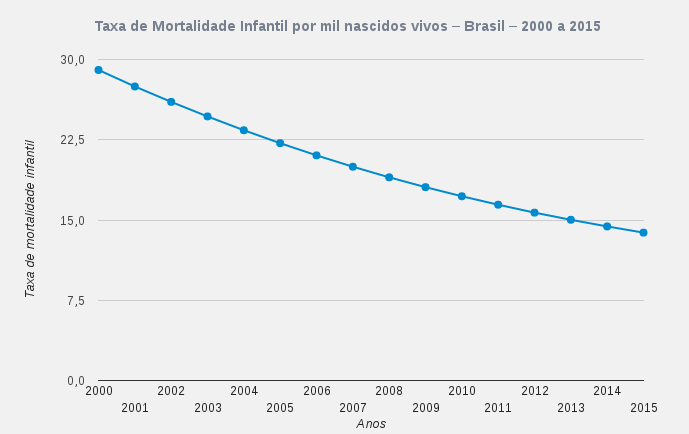
\includegraphics[width=\linewidth]{mortalidade_infantil.png}
\end{figure}
Fonte: \cite{ibgeMortalidade}
\end{center}

Apesar da significativa redução através dos anos, o Brasil ainda precisa melhorar
muito em relação aos países de primeiro mundo. A taxa de mortalidade atual (13,82/1000 nascidos vivos)
é cerca de três a seis vezes maior que a de países desenvolvidos, como Japão, Canadá e Alemanha que
apresentam taxa de 3 a 10/1000 nascidos vivos.

Essas mortes precoces podem ser evitadas em sua maioria, com o fácil e rápido acesso a serviços
qualificados de saúde e com a prevenção de doenças conhecidas. Além disso, fatores externos também
contribuem para a mudança desta taxa, como acesso ao  saneamento básico, taxa de fecundidade,
segurança alimentar e nutricional, grau de instrução das mulheres, avanço das tecnologias médicas,
em especial a imunização e terapia de reidratação oral, prevalência do aleitamento materno,
entre outros \cite{lansky2009mortalidade}, \cite{frias2008politicas}.

Para entender melhor a dinâmica da taxa de mortalidade infantil, estudar como cada um destes elementos
afeta a mesma torna-se uma necessidade.
